\documentclass[english]{article}
\usepackage[OT1]{fontenc}
\usepackage{geometry}
\geometry{verbose,tmargin=2.5cm,bmargin=2.5cm,lmargin=2.5cm,rmargin=2.5cm}
\usepackage{float}
\usepackage{graphicx}
\usepackage{babel}

\usepackage{tikz}
\usepackage{pgfplots}
\usepackage{circuitikz}
\usetikzlibrary{arrows, positioning, calc,shapes}
\usepackage{enumitem}
\usepackage{hyperref}
\usepackage{nameref}% Only if hyperref isn't loaded

\usepackage{amsmath,amssymb}
\makeatletter
\newsavebox\myboxA
\newsavebox\myboxB
\newlength\mylenA

\newcommand*\xoverline[2][0.75]{%
    \sbox{\myboxA}{$\m@th#2$}%
    \setbox\myboxB\null% Phantom box
    \ht\myboxB=\ht\myboxA%
    \dp\myboxB=\dp\myboxA%
    \wd\myboxB=#1\wd\myboxA% Scale phantom
    \sbox\myboxB{$\m@th\overline{\copy\myboxB}$}%  Overlined phantom
    \setlength\mylenA{\the\wd\myboxA}%   calc width diff
    \addtolength\mylenA{-\the\wd\myboxB}%
    \ifdim\wd\myboxB<\wd\myboxA%
       \rlap{\hskip 0.5\mylenA\usebox\myboxB}{\usebox\myboxA}%
    \else
        \hskip -0.5\mylenA\rlap{\usebox\myboxA}{\hskip 0.5\mylenA\usebox\myboxB}%
    \fi}
    
\makeatletter


\begin{document}

\title{Design of digital integrated systems: optimization of a 16 bit Brent-Kung adder}
\author{Matthijs Van keirsbilck}

\maketitle

\section{Schematic and optimisation}

\begin{enumerate}
    \item \label{itm:first} This is a numbered item
    \item Another numbered item \label{itm:second}
    \item \label{itm:third} Same as \ref{itm:first}
\end{enumerate}
Cross-referencing items \ref{itm:second} and \ref{itm:third}.


\subsection{Optimisation}

\begin{enumerate}
\item Architectural \label{itm:arch}

\begin{itemize}
\item To remove inverters from the critical path, as a first attempt, the DotProducts were replaced with equivalent NAND-based operators. This was quite easy to implement, as only one type of DotProduct was needed, and provided a significant increase in performance. 
  
\item Even better performance was reached by using AOI and OAI- based DotOperators, where the DotProducts are replaced with DotProductNormal and DotProductInverse. In the rest of the report, that architecture will be described.
In the top half of the structure, most DotProducts are full-size (both generate and propagate).
Lower down, the propapagate signal is often not use, so some gates can be removed, leading to lower power.
As the number of normal/inverting stages is not equal for all paths, some special operators are required as well. DotProductSimpleNormalHighInvertedLow for example is a dotproduct that doesn't generate a propagate signal, and takes as input the $P_h$ and $G_h$ as well as \xoverline{G_l}.
In total, there are six different DotOperators (with their abbreviations between brackets):

\begin{enumerate}
\item DotOperatorNormalIn ('DON')
\item DotOperatorInvertedIn ('DOI')
\item DotOperatorSimpleNormalIn ('DOSN')
\item DotOperatorSimpleInvertedIn ('DOSI')
\item DotOperatorSimpleNormalHighInvertedLow ('DOSNHIL')
\item DotOperatorSimpleInvertedHighNormalLow ('DOSIHNL')
\end{enumerate}
See the circuit for the structure \ref{modifiedAdderSchematic}.

\item An efficient 6-transistor implementation of the XOR gate (based on transmission gates) decreases delay by a lot, because of less transistors, faster switching speed and reduced load on the critical path. Because only one consecutive transmission gate stage is used, output isn't degraded much and no buffers are needed (see \cite{website:xorTransmissionGate}).

\begin{figure}[H]
\begin{centering}
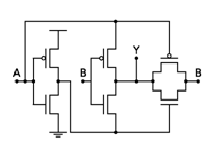
\includegraphics{figures/efficientXOR.png}
\par\end{centering}
\caption{Schematic of the optimised XOR gate}
\label{adderSchematic}
\end{figure}

\item The building blocks (AOI, OAI, NAND, XOR, NOT) were optimized in size to take into account that some transistors were placed in parallel or in series, respectively increasing or reducing the current in that branch. See Sizing.

\item If buffers in the structure buffer a large subcircuit, they will significantly reduce the load on critical path, making it faster. The buffers increase the delay of the path they are placed on, however. This could make those paths the new bottlenecks. The only two minimum-sized buffers that were introduced are situated quite low in the hierarchy so that they don't increase the delays of too many paths (see Figure \ref{adderSchematic}).

\end{itemize} %end arch


\item Sizing \label{itm:sizing}

For achieving maximum speed, widths of some transistors were changed by some scalar factor:
\begin{itemize}
\item pMOSscalar: normally, pMOS devices are sized about twice as large as nMos devices to keep switching symmetrical (this is needed due to lower mobility of holes compared to electron)s. For this adder design, however, lower pMOS width means lower capacitance, and this results in faster switching speeds. Too low values mean that the asymmetricalities will increase delay, too high values increase the capacitive load and reduce delay as well. This trade-off resulted in an optimal pMOS sizing of 1.6 times the nMOS size.
\item seriesScalar: in for example a NAND gate, the 2 nMOS devices are placed in series between output and ground. This results in higher series resistance for the current flow and an extra capacitive node that needs to be drained. Series devices can provide less current than a single device due to these reasons, while devices in parallel can provide double the current. To compensate for these effects, transistors in series configurations are scaled by a factor of seriesScalar.
\item critBasePath: The top right half of the adder (until input7, and DotOperator(7\_0)) is very important for all critical paths. This scalar modifies the widths of transistors in this area.
\item critPath1: The most critical path (6 DotOperators), that runs diagonally from input0 to s15. Increasing its size improves speed, but also increases loading.
\item critPath2: The secondmost critical path. If the first critical path is sized large enough, it will no longer have the largest delay, and this second critical path needs to be scaled as well. This increases the load on the first critical path, increasing its delay. A balance needs to be found.
\item XORScalar: some of the paths are more critical than others. For precise adjustments to the path delay, the XOR gates at the end of the path can work faster if they are scaled, without modifying the whole path (which would have a large effect on the loading as well). The most important paths at s15 and s9 were scaled this way.
\item VDD: this reduces the DC power consumtion and the switching energy, but increases the delay. When a good Energy-Delay Product (EDP) is reached, scaling the voltage reduces power consumption. Vdd= 0.93V was the lowest supply voltage where the circuit still fulfilled the specifications.
 
\end{itemize} % end sizing


\end{enumerate} %end architectural/sizing 






\section{Results}
Two different architectures are shown, one that targets maximum possible speed, and another that targets minimum power with a delay constraint of 650ps.
To measure these results, one test file was run for each path. Propagation of an input change through all important critical paths were simulated throuth a '.vec' file for each path (thanks to Bob Vanhoof for providing some basic test files). 
The shown delay, switching energy, and EDP are the worst (maximum) delay of all test cases (not necessarily the same one). The DC power obviously remains constant for a given architecture.

\subsection{Max speed}
\begin{table}[h]
\centering
\begin{tabular}{ |l|r| }
\hline
scalar	& value \\
\hline
 pMOSscalar		& 1.6 \\
 seriesScalar   & 2.6 \\
 critBase   	& 1.4 \\
 critPath1   	& 1.8 \\
 critPath2    	& 1.1 \\
\hline
\end{tabular}
\caption{Size Scaling factors for maximum speed}
\label{SpeedScalars}
\end{table}

\begin{table}[h]
\centering
\begin{tabular}{ |l|r| }
\hline
Supply	&	1 V \\
Worst Case delay &            511 ps  \\
Worst Case Switching energy & 135 fJ \\
Worst Case DC power &        1.73 nW  \\
Worst Case EDP &              69045 ps*fJ \\
\hline
\end{tabular}
\caption{Performance of the circuit tuned for maximum speed}
\label{SpeedPerformance}
\end{table}

\subsection{Minimum Power @ 650ps}

\begin{table}[h]
\centering
\begin{tabular}{ |l|r| }
\hline
scalar	& value \\
\hline
 pMOSscalar		& 1 \\
 seriesScalar   & 2.6 \\
 critBase   	& 1 \\
 critPath1   	& 1.5 \\
 critPath2    	& 1 \\
\hline
\end{tabular}
\caption{scaling factors for minimum power}
\label{MinPowerScalars}
\end{table}

\begin{table}[h]
\centering
\begin{tabular}{ |l|r| }
\hline
Supply	&	0.93 V \\
Worst Case delay &            648 ps \\
Worst Case Switching energy & 113 fJ\\
Worst Case DC power &        1.936 nW \\
Worst Case EDP &              733578 ps*fJ \\
\hline
\end{tabular}
\caption{Final performance of the circuit tuned for minimum power and 650ps delay}
\label{PowerPerformance}
\end{table}   


\subsection{performance with pMOS width = 1.0}

For the maximum speed circuit, the delay goes up when pMOSscalar is lowered too much, but this is not the case for the minimum power circuit (the only difference between the circuits is the sizing of the critical paths).
For the minimum power circuit, it is very surprising that the extremely low width of pMOS transistors doesn't increase delay (since it introduces asymmetricalities), and seems to improve the circuit by a large margin (EDP of 55k while it was \textgreater 70k before). The reason the simulation gave these results might be because the test cases don't cover every possible switching event. 
Therefore, the simulation above, with more conservative pMOS sizes obtined from the maximum speed optimizations is considered to show the actual performance of the circuit.

\begin{table}[h]
\centering
\begin{tabular}{ |l|r| }
\hline
Supply	&	0.94 V \\
Worst Case delay &            645.5 ps \\
Worst Case Switching energy & 85.14 fJ \\
Worst Case DC power &         1.7786 nW \\
Worst Case EDP &              54963 ps*fJ\*fJ \\
\hline
\end{tabular}
\caption{Performance tuned for minimum power and 650ps delay, with pMOSscalar = 1.0}
\label{PowerPerformancePmos1.0}
\end{table}



\newpage{}


\subsection{Schematic}

\begin{figure}[H]
\begin{centering}
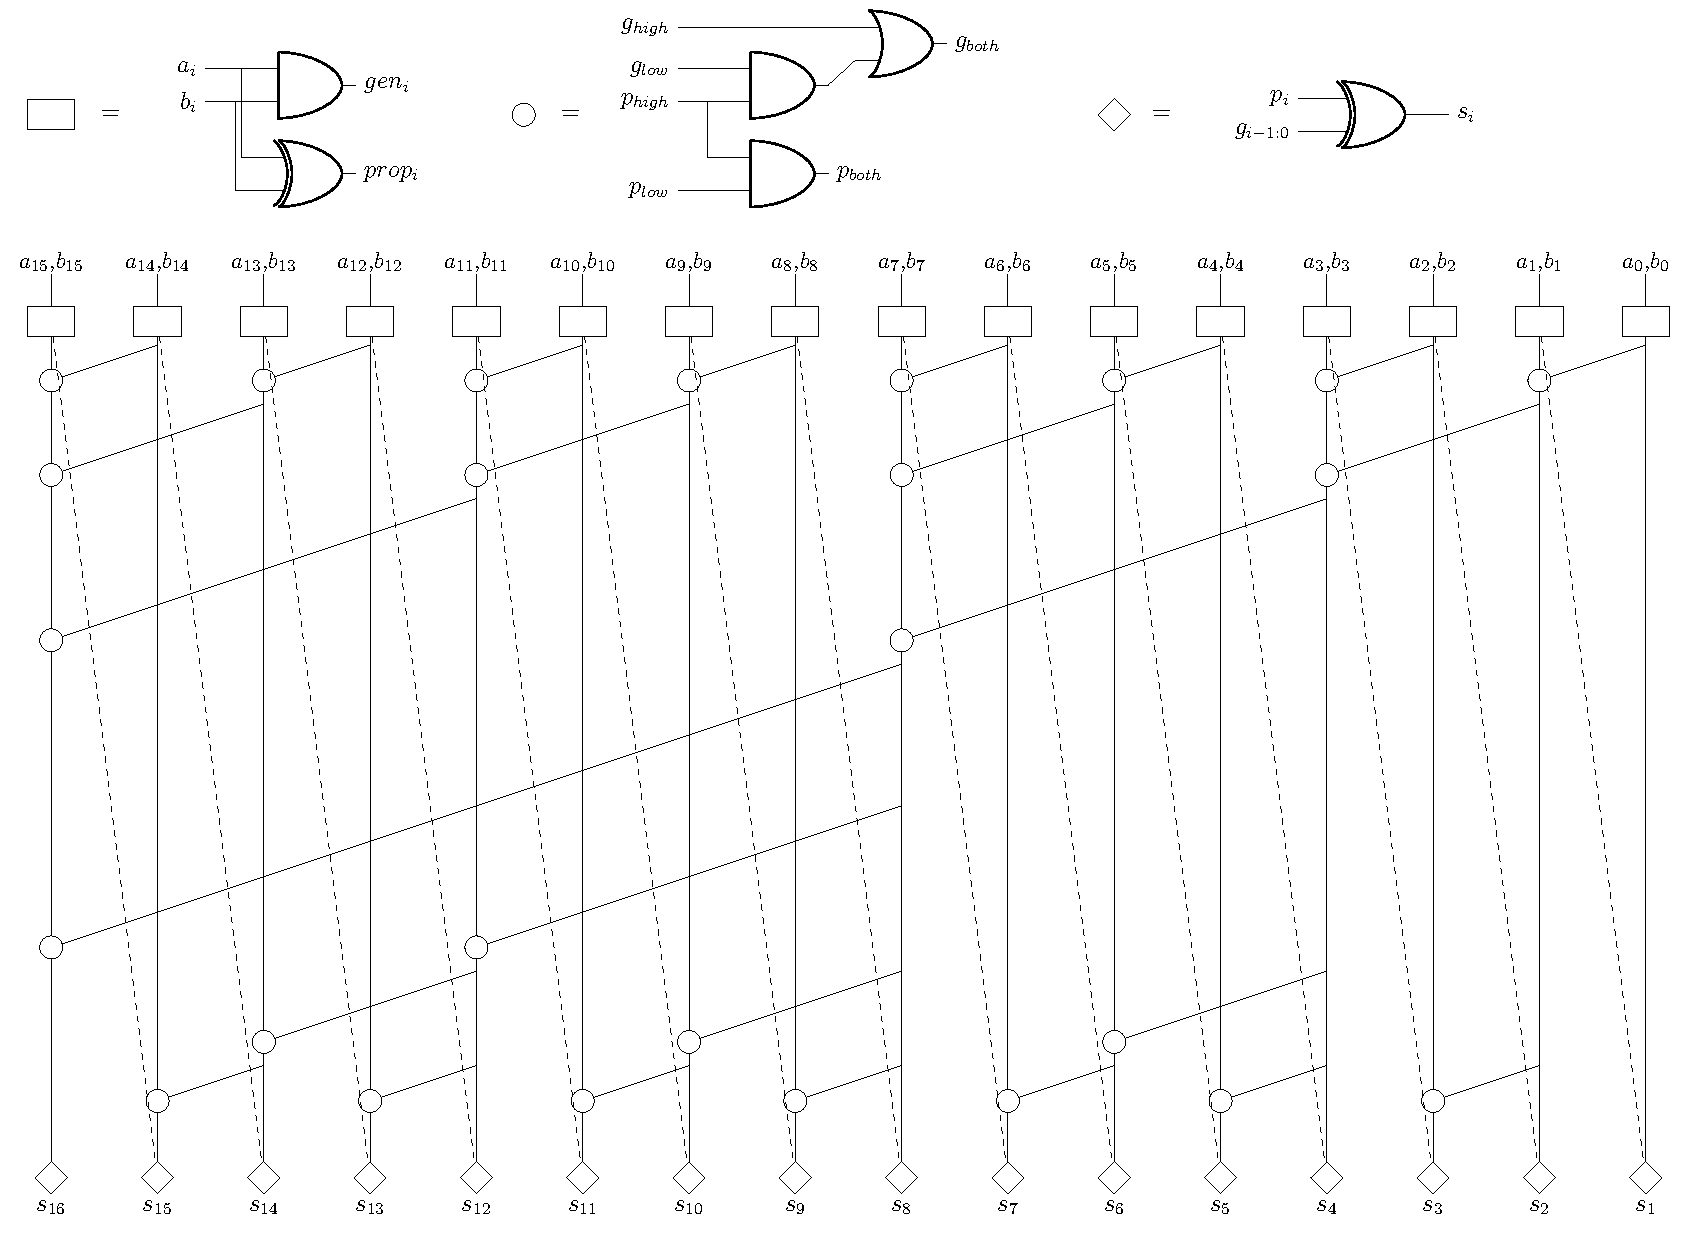
\includegraphics[angle=90,width=0.9\textwidth]{figures/modifiedBrentKung_tex}
\par\end{centering}
\caption{Schematic of the optimised adder}
\label{modifiedAdderSchematic}
\end{figure}

\begin{figure}[H]
\begin{centering}
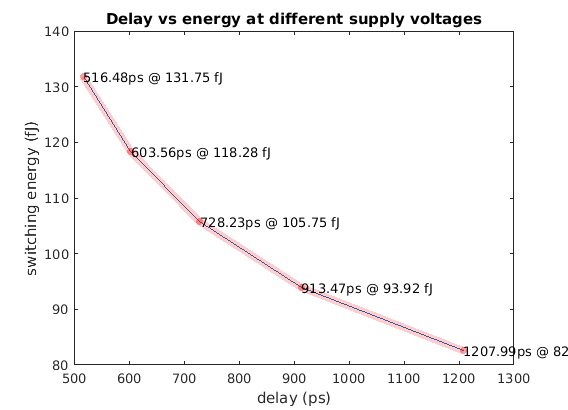
\includegraphics[width=0.9\textwidth]{figures/EDPlabeled.png}
\par\end{centering}
\caption{EDP of the optimised adder}
\label{adderSchematic}
\end{figure}

\medskip

\begin{thebibliography}{9}

\bibitem{website:xorTransmissionGate}
Universitat Hamburg
\textit{CMOS transmission-gate XOR gate}
accessed: 28/10/2016
\\\texttt{https://tams-www.informatik.uni-hamburg.de/applets/hades/webdemos/05-switched/40-cmos/xor-tgate.html}

\bibitem{adderOverview}
Noel Daniel Gundi
\textit{Implementation of 32 bit Brent-Kung adder using complementary pass transistor logic}
accessed: 28/10/2016
\\\texttt{https://shareok.org/bitstream/handle/11244/25747/Gundi\_okstate\_0664M\_13905.pdf?sequence=1}

\end{thebibliography}
 



\end{document}
